%% --------------------------------------------------------------------------
% LaTeX template for the XLI CILAMCE.
%
% This latex document tries to copy the Microsoft Word template.
% --------------------------------------------------------------------------
\documentclass[a4paper,10pt]{book}

% PACKAGES USED - packages that need to be previously installed on your computer
\usepackage[lmargin=2.5cm, rmargin=2.5cm, tmargin=2.5cm, bmargin=2.5cm ]{geometry}
\usepackage{graphicx}
\usepackage{times}
\usepackage{indentfirst}
\usepackage{fancyhdr}
\usepackage{titlesec}
\usepackage[english]{babel}
\usepackage{parskip} 
\usepackage{setspace}



%%%%%%%%%%%%%%%%%%%%%%%%%%%%%%%%%%%%%%%%%%%%%%%%%%%%%%%%%%%%%%%%%
%%%%%%%%%%%%%%%%%%%%%%%%%%%%%%%%%%%%%%%%%%%%%%%%%%%%%%%%%%%%%%%%%
%%% My Additional Packages
%%%%%%%%%%%%%%%%%%%%%%%%%%%%%%%%%%%%%%%%%%%%%%%%%%%%%%%%%%%%%%%%%
\usepackage[utf8]{inputenc}
%\usepackage{amssymb} %Mathematics
%\usepackage{amsfonts}%Mathematics
%\usepackage{amsmath,amscd}%Mathematics
%\usepackage{amsthm}%Mathematics
%\usepackage{mathrsfs}%Mathematics font
%\usepackage{xspace}
%\usepackage{booktabs}
%\usepackage{stmaryrd}%Particular Brackets
%\usepackage{graphicx} %Tables and Figures
%\usepackage{subfigure}
%\usepackage{url}
\usepackage{hyperref}
\usepackage{cleveref}
\usepackage{./pkg-crefNames}
\usepackage[labelsep=period]{caption}

%BibTeX compatible with the CILAMCE format
\usepackage[numbers,sort&compress]{natbib}

\setlength{\bibsep}{0pt plus 0.3ex}

\renewcommand*{\bibfont}{\small}

\makeatletter
\renewcommand\bibsection
{
  \section*{References}
}



\renewenvironment{thebibliography}[1]
      {\section*{Referêcias}%
       \@mkboth{\MakeUppercase\refname}{\MakeUppercase\refname}%
       \list{\@biblabel{\@arabic\c@enumiv}}%
            {\settowidth\labelwidth{\@biblabel{#1}}%
             \leftmargin\labelwidth
             \advance\leftmargin-10pt% change 20 pt according to your needs
             \advance\leftmargin\labelsep
             \setlength\itemindent{10pt}% change using the inverse of the length used before
             \@openbib@code
             \usecounter{enumiv}%
             \let\p@enumiv\@empty
             \renewcommand\theenumiv{\@arabic\c@enumiv}}%
       \sloppy
       \clubpenalty4000
       \@clubpenalty \clubpenalty
       \widowpenalty4000%
       \sfcode`\.\@m}
      {\def\@noitemerr
        {\@latex@warning{Empty `thebibliography' environment}}%
       \endlist}
\renewcommand\newblock{\hskip .11em\@plus.33em\@minus.07em}
\makeatother




\makeatother
\bibliographystyle{bib-cilamce}
%\bibliographystyle{plain}


%%%%%%%%%%%%%%%%%%%%%%%%%%%%%%%%%%%%%%%%%%%%%%%%%%%%%%%%%%%%%%%%%
%%%%%%%%%%%%%%%%%%%%%%%%%%%%%%%%%%%%%%%%%%%%%%%%%%%%%%%%%%%%%%%%%

% CONFIGURATION
\renewcommand*\arraystretch{1.5}
\renewcommand*\thesection{\arabic{section}}
%\hyphenpenalty=10000 % You can uncomment this to avoid hyphenization
\titleformat*{\section}{\large\bfseries}
\titleformat*{\subsection}{\bfseries}
\titlespacing\section{0pt}{20pt plus 2pt minus 2pt}{12pt plus 2pt minus 2pt}
\titlespacing\subsection{0pt}{20pt plus 0pt minus 0pt}{12pt plus 0pt minus 0pt}
\setlength{\parskip}{0pt} % Spacing between paragraphs
\setlength{\parindent}{0.75cm} % Paragraph identation
\setlength\abovecaptionskip{6pt}

% --------------------------------------------------------------------------
% DO NOT EDIT - SPECIAL HEADINGS OF XLI CILAMCE
% --------------------------------------------------------------------------
\fancypagestyle{first}
{
\fancyhf{}
\fancyfoot[RO]{\footnotesize \textit{CILAMCE 2020 \\
Proceedings of the XLI Ibero-Latin-American Congress on Computational Methods in Engineering, ABMEC.\\
Foz do Iguaçu/PR, Brazil, November 16-19, 2020}}
\renewcommand{\headrulewidth}{.0pt}
\renewcommand{\footrulewidth}{.5pt}
}

\pagestyle{fancy}
\fancyhf{}
\fancyhead[RO,LE]{}

\fancyfoot[RO]{\footnotesize \textit{CILAMCE 2020 \\
Proceedings of the XLI Ibero-Latin-American Congress on Computational Methods in Engineering, ABMEC.\\
Foz do Iguaçu/PR, Brazil, November 16-19, 2020}}

\fancyfoot[LE]{\footnotesize \textit{CILAMCE 2020 \\
Proceedings of the XLI Ibero-Latin-American Congress on Computational Methods in Engineering, ABMEC.\\
Foz do Iguaçu/PR, Brazil, November 16-19, 2020}}

\renewcommand{\headrulewidth}{.5pt}
\renewcommand{\footrulewidth}{.5pt}

% --------------------------------------------------------------------------
% PLEASE, EDIT THIS!
\fancyhead[LE]{\footnotesize \textit{CILAMCE 2020 Previsão da resistência à compressão do concreto com técnicas de aprendizado de máquina}}
\fancyhead[RO]{\footnotesize \textit{P. Moreira, V. Silva}}
% --------------------------------------------------------------------------

\begin{document}\thispagestyle{first}

\renewcommand{\figurename}{Figura}
\renewcommand{\tablename}{Tabela}

% --------------------------------------------------------------------------
% DO NOT EDIT - LOGO OF XLI CILAMCE
% --------------------------------------------------------------------------

\begin{figure}[ht!]
\vspace{-30pt}
\flushright
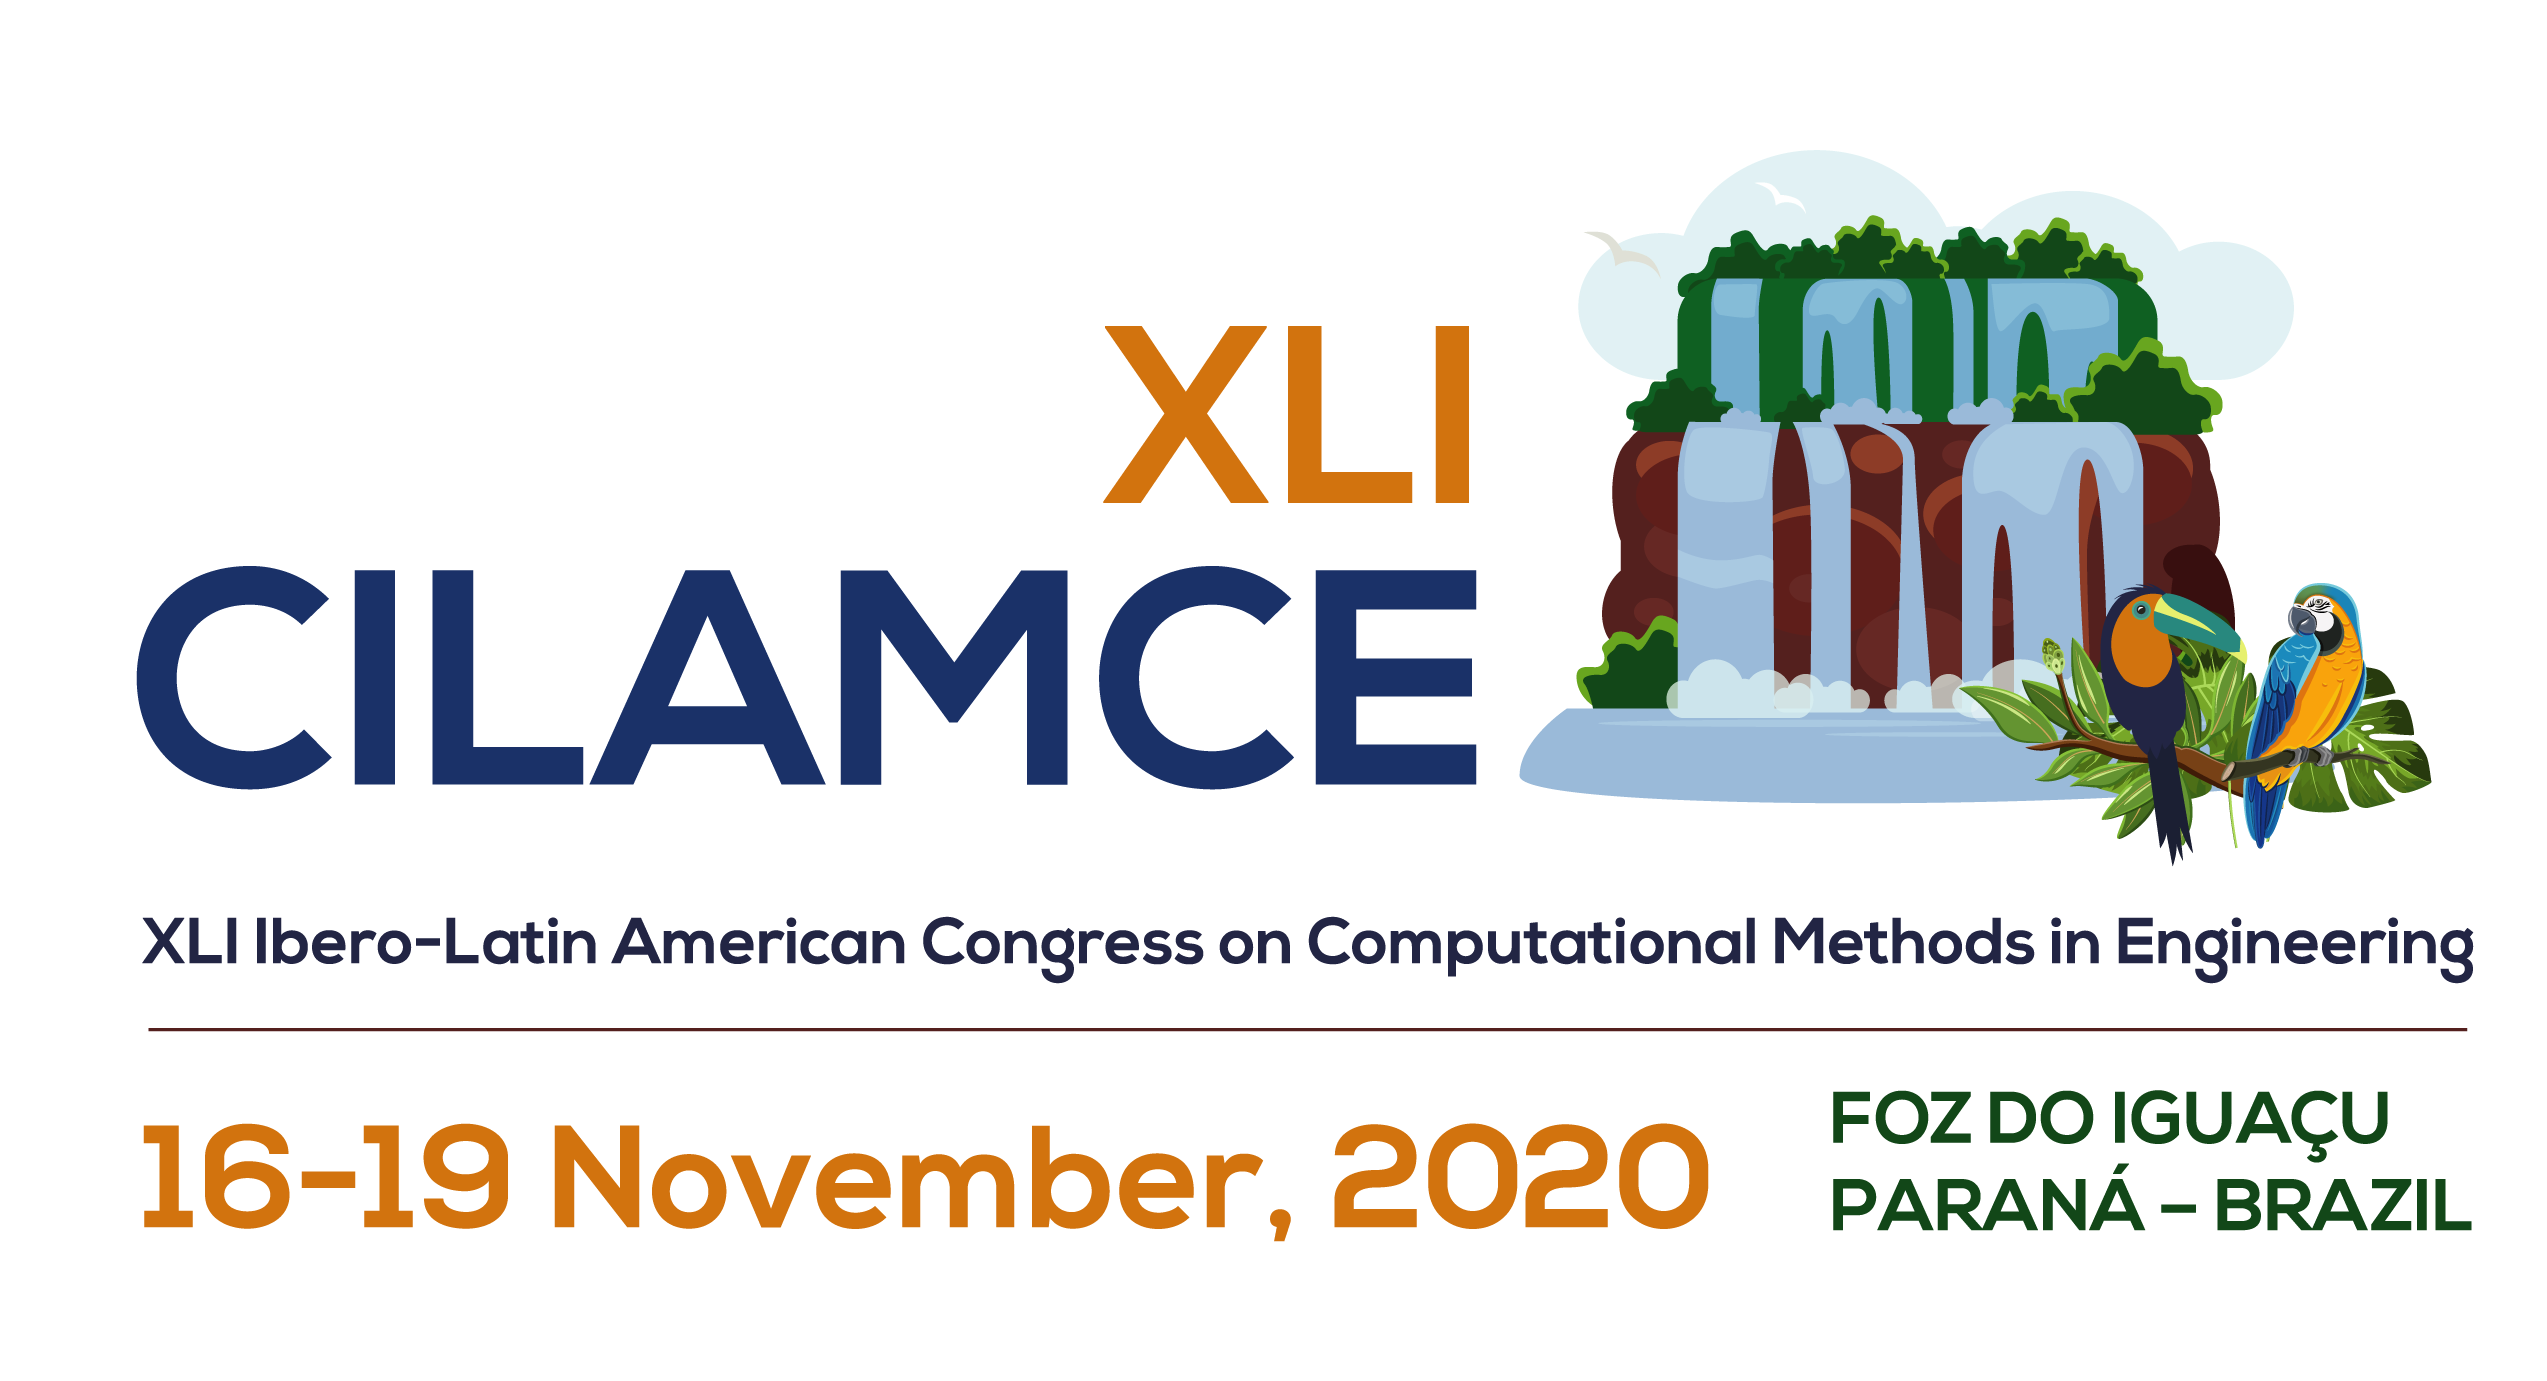
\includegraphics[width=5.5cm]{Figures/logoCILAMCE2020.png}
%scale=0.25
\end{figure}

% --------------------------------------------------------------------------
% TITLE OF PAPER
% --------------------------------------------------------------------------

\noindent
\textbf{\Large
Previsão da resistência à compressão do concreto com técnicas de aprendizado de máquina} 
\vspace{14pt} % <- keep this vertical space!

% --------------------------------------------------------------------------
% AUTHORS
% --------------------------------------------------------------------------

\noindent Pedro B. A. Moreira$^1$, Victor M. Silva$^2$

\vspace{14pt} % <- keep this vertical space!

\noindent $^1$\textit{Estudante, Engenharia Civil, Universidade Veiga de Almeida}

\noindent \textit{Avenida das Américas, 22631-004, Rio de Janeiro, Brazil}

\noindent \textit{pedrobermoreira@gmail.com}

\noindent $^2$\textit{Professor, Engenharias, IBMEC/RJ}

\noindent \textit{Avenida Armando Lombardi 940, 22640-000, Rio de Janeiro, Brazil}

\noindent \textit{victor.silva@professores.ibmec.edu.br}


\vspace{18pt} % <- keep this vertical space!

% --------------------------------------------------------------------------
% ABSTRACT
% --------------------------------------------------------------------------

\noindent \textbf{Resumo.}
A resistência à compressão é a principal característica do concreto. A previsão correta deste parâmetro significa redução de custo e tempo. Este trabalho construiu modelos preditivos para 6 diferentes idades de amostras de concreto. Foi utilizado um conjunto de 1.030 amostras de estudos anteriores, com 9 variáveis. Outras 6 variáveis ​​foram adicionadas para representar as proporções dos ingredientes principais em cada amostra. Os modelos preditivos foram desenvolvidos em linguagem {\it R}, utilizando o algoritmo {\it Parallel Random Forest} e a técnica de validação cruzada repetida para otimizar os parâmetros. Os resultados foram compatíveis com outros estudos usando o mesmo conjunto de dados. O modelo mais importante, de 28 dias, obteve um erro quadrático médio ({\it RMSE}) de 4,717. O modelo de 3 dias obteve o melhor resultado, {\it RMSE} de 3,310. O trabalho mostrou que a resistência à compressão do concreto pode ser prevista. Criar um modelo para cada idade permitiu obter resultados compatíveis com os dados disponíveis em cada idade. Foi uma alternativa promissora, pois bons resultados foram alcançados treinando com apenas um algoritmo. Este trabalho facilita a exploração e novos esforços para prever a resistência à compressão do concreto, pode ser usado como linha de base para diferentes algoritmos ou a combinação de vários.

\vspace{18pt} % <- keep this vertical space!

\noindent \textbf{Palavras-chave:} Concreto, Resistência à compressão, Aprendizado de Máquina, Previsão, {\it Parallel Random Forest}

% --------------------------------------------------------------------------
\section{Introdução}\label{sec:introduction}
% --------------------------------------------------------------------------


A resistência à compressão é a principal característica do concreto, medida por ensaios de padrões internacionais que consistem na quebra de corpos de prova \cite{Gambhir1990}. A medição aos 28 dias é obrigatória e representa a classe do concreto. Saber com antecedência o resultado em uma determinada idade, com base nas proporções de seus ingredientes, é de grande interesse para fabricantes de concreto, construtoras e engenheiros civis.
 
A resistência à compressão é uma função não linear de seus ingredientes e idade, dificultando o estabelecimento de uma fórmula analítica, embora algumas já tenham sido propostas por \citet{Hasan2011} e  \citet{Kabir2012}. Porém, a maioria dos estudos construiu modelos incluindo a idade como característica junto com os ingredientes, mas devido à não linearidade entre a resistência à compressão e a idade, constatamos a necessidade de maiores investigações de modelos que separem a idade e analisem apenas os ingredientes.

Portanto, o presente estudo visa a construção de modelos preditivos da resistência à compressão do concreto em diferentes idades utilizando apenas seus ingredientes como características.


% --------------------------------------------------------------------------
\section{Trabalhos Relacionados}\label{sec:RelatedWork}
% --------------------------------------------------------------------------


\citet{Yeh1998} demonstrou a possibilidade de usar Redes Neurais Artificiais para prever a resistência à compressão do concreto, concluindo que é um método mais preciso do que os modelos de regressão. Neste estudo, mais de 1.000 amostras de concreto foram coletadas de 17 fontes diferentes. Este conjunto de dados foi posteriormente utilizado em vários estudos sobre concreto, alguns dos quais são mencionados a seguir.

\citet{Alshamiri2020} propôs um novo método, {\it Regularized Extreme Learning Machine} ({\it RELM}) para treinar modelos de Redes Neurais Artificiais para predizer a resistência à compressão. Os resultados foram comparados com vários algoritmos conhecidos rodando no mesmo conjunto de dados, incluindo individual e {\it ensembles}, e o modelo proposto teve o melhor resultado de longe.

\citet{Hameed2020} compara modelos de Rede Neural Artificial com Regressão Linear Múltipla para prever a força de resistência à compressão e descobriu que os modelos de Rede Neural Artificial obtêm muito mais precisão do que a Regressão Linear Múltipla.

Além desses estudos publicados, agora é muito comum publicar projetos pessoais em páginas da web. Por fácil acesso a este banco de dados e o crescente interesse em ciência de dados e aprendizado de máquina, alguns estudos não publicados usando esse mesmo banco de dados incluem \citet{Modukuru2020}, \citet{Raj2018}, \citet{Abban2016} e  \citet{Pierobon2018}. No geral, todos seguiram as etapas padrão no desenvolvimento de modelos de aprendizado de máquina, os dois primeiros usando o pacote {\it scikit-learn} em linguagem {\it python} desenvolvido por  \citet{pedregosa2011scikit} e os dois últimos usaram o pacote {\it caret} desenvolvido por \citet{caret} em linguagem {\it R} \cite{RCore}.

Ao final deste trabalho, na seção de discussão e conclusão, os resultados encontrados neste trabalho são comparados com todos esses estudos relacionados.



% --------------------------------------------------------------------------
\section{Metodologia}\label{sec:MaterialsAndMethods}
% --------------------------------------------------------------------------

% --------------------------------------------------------------------------
\subsection{Materiais e reprodutibilidade} \label{subsec:materialsandreproducibility}
% --------------------------------------------------------------------------

A metodologia foi realizada no software {\it RStudio} \cite{RStudio}, um ambiente virtual integrado para desenvolvimento de código em linguagem {\it R} \cite{RCore}. Ao longo do processo, todo o código executado foi documentado na mesma ordem de sua execução e enviado para o repositório online hospedado no {\it github} \cite{github}. O repositório contém uma versão estendida deste trabalho, incluindo todo o código, pacotes necessários e versões. Para garantir a reprodutibilidade, sempre que um código utilizou operações probabilísticas, um {\it seed} foi definido antes de sua execução, garantindo a consistência dos resultados ao rodar em outra máquina.

 

% --------------------------------------------------------------------------
\subsection{Conjunto de dados} \label{subsec:dataset}
% --------------------------------------------------------------------------
Os dados foram baixados do site da Universidade da Califórnia em Irvine  \cite{downloadData}. No total, são 1.030 linhas com 9 colunas. Cada linha representa uma amostra com as variáveis: resistência à compressão, idade e 7 ingredientes (água, cimento, agregado miúdo, agregado graúdo, cinza volante, escória de alto-forno e superplastificantes).

% --------------------------------------------------------------------------
\subsection{Preparação dos dados} \label{subsec:datapreparation}
% --------------------------------------------------------------------------

Os trabalhos relacionados utilizaram o conjunto de dados em sua totalidade ou realizaram um mínimo de preparação. De forma diferente, neste trabalho uma etapa específica foi dedicada apenas a limpar as amostras e prepará-las para as próximas etapas. As principais etapas executadas nesta seção estão listadas abaixo:

\begin{enumerate}
\item Amostras duplicadas foram removidas;

\item As amostras foram agregadas e identificadas (com um nova coluna de {\it ID}) pelas configurações de proporção dos ingredientes, independente de sua idade;

\item Idades de 90, 91 e 100 dias foram fundidas em uma única categoria de 100 dias. Essa etapa foi realizada com o seguinte desenvolvimento: primeiro, traçando e analisando o {\it boxplot} agrupado por idade na Fig. \ref{fig:boxplot} mostrou que as amostras de 90, 91 e 100 dias têm concentrações distintas de valores de resistência à compressão. Em seguida, uma análise de componentes principais ({\it PCA}) dos ingredientes foi feita na Fig. \ref{fig:pca}, mostrando que as combinações de ingredientes dessas idades são muito distintas. Como são idades muito próximas, é razoável que possamos juntar essas idades sem qualquer prejuízo nas previsões. Por fim, a marca dos 100 dias foi escolhida porque a análise de amostras que continham dados em pelo menos cinco idades diferentes mostrou que a resistência à compressão tende a aumentar com o tempo. Portanto, uma idade mais avançada tende a fornecer resultados mais conservadores.


\item Após juntar as idades de 90, 91 e 100 dias, foram retiradas as idades com frequência menor que 50, restando apenas as idades de 3, 7, 14, 28, 56 e 100 dias;

\item Para amostras com o mesmo {\it ID} e a mesma idade, mas com diferentes valores de resistência à compressão, os dados foram combinados em uma única linha para cada combinação de {\it ID} e idade, contendo uma média das resistências à compressão;

\item Foram mantidos apenas os {\it ID}s que possuem dados na marca de 28 dias;

\item Adição de 6 novas variáveis contínuas que foram usados nos modelos de predição, representando as proporções entre os ingredientes principais (água / cimento, agregado miúdo / cimento, agregado graúdo / cimento, agregado miúdo / agregado graúdo, água / agregado graúdo e água / agregado miúdo);

\item Acréscimo de 2 novas variáveis ​​categóricas utilizadas para visualizar a distribuição das amostras (classe do concreto e traço aproximado).
\end{enumerate}

\begin{figure}[!ht]
\begin{center}
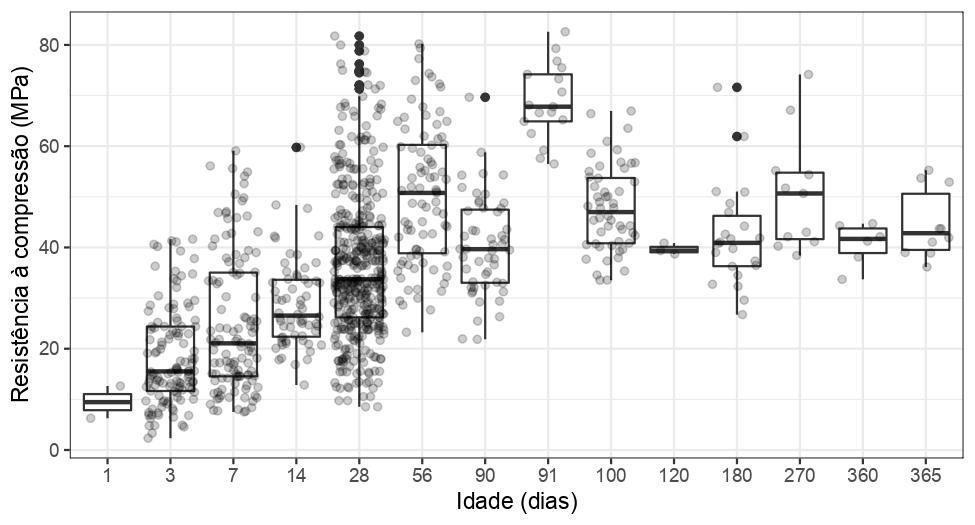
\includegraphics[scale=0.8]{Figures/boxplot_PT.jpg}
\vspace{12pt}
\caption{{\it Boxplot} - resistência à compressão agrupada por idade}
\label{fig:boxplot}
\end{center}
\end{figure}
\vspace{8pt}

\begin{figure}[!ht]
\begin{center}
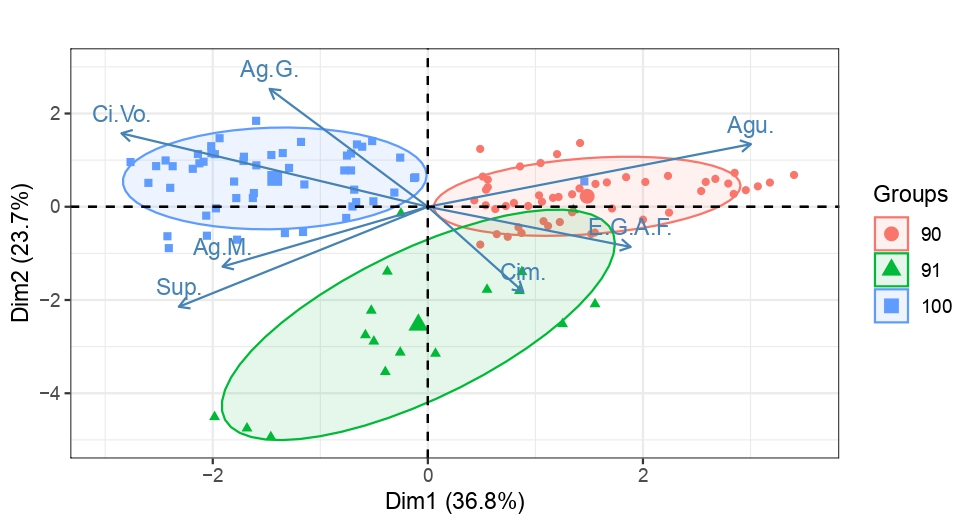
\includegraphics[scale=0.8]{Figures/pca-90-91-100_PT.jpg}
\vspace{12pt}
\caption{Análise de componente principal - 90, 91 e 100 dias}
\label{fig:pca}
\end{center}
\end{figure}
\vspace{8pt}

Após essas manipulações, o número final de amostras foi reduzido de 1.030 linhas para 916 linhas, com 416 configurações de ingredientes diferentes ({\it IDs}). Um arquivo {\it xls} dos dados neste momento está disponível para download no repositório no github  \cite{github}.


% --------------------------------------------------------------------------
\subsection{Visualização dos dados} \label{subsec:datavisualization}
% --------------------------------------------------------------------------

Além dos gráficos já apresentados, vários outros gráficos e tabelas foram construídos para realizar a exploração e visualização das amostras preparadas na etapa anterior, dentre elas:

\begin{itemize}

\item Estatística descritiva das variáveis contínuas e categóricas;

\item Distribuição das variáveis em relação à resistência à compressão;

\item Correlação entre as variáveis agrupadas por idade;

\item Relação entre o traço aproximado e a resistência à compressão;

\item Relação entre os principais ingredientes do concreto e a resistência à compressão;

\item Análise de componentes principais ({\it PCA}) dos ingredientes.

\end{itemize}

Os gráficos para da estatística descritiva das variáveis categóricas são apresentados, na Fig. \ref{fig:categorical}.

\begin{figure}[!ht]
\begin{center}
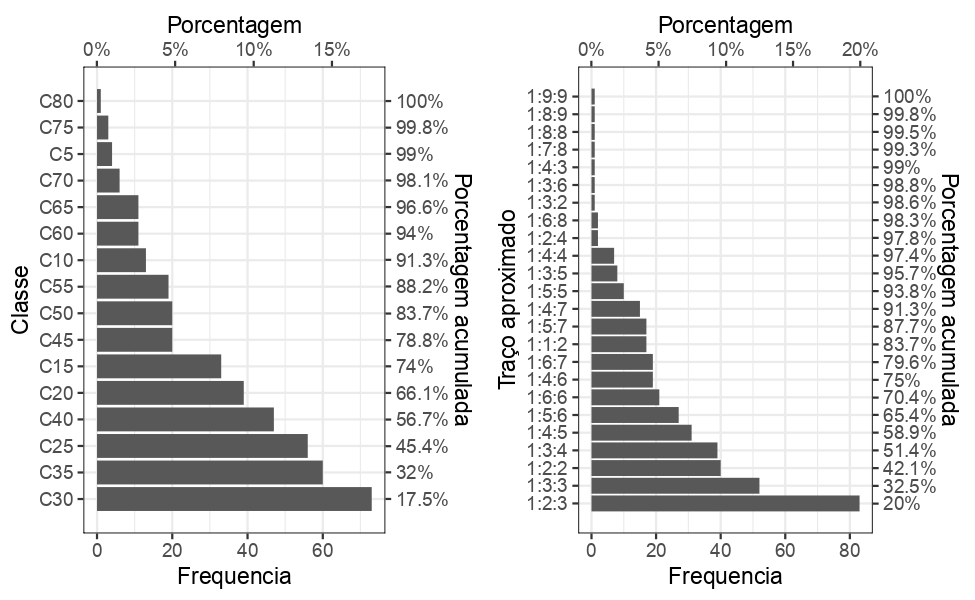
\includegraphics[scale=0.8]{Figures/stat-summ-categorical_PT.jpg}
\vspace{12pt}
\caption{Estatística descritiva das variáveis categóricas}
\label{fig:categorical}
\end{center}
\end{figure}
\vspace{8pt}

% --------------------------------------------------------------------------
\subsection{Pré-processamento e separação dos dados} \label{subsec:preprocessing}
% --------------------------------------------------------------------------

 O principal pacote usado para construir os modelos de aprendizado de máquina foi o pacote {\it Caret}  \cite{caret}. Ele fornece todas as funcionalidades e utilitários para construir modelos de previsão para qualquer conjunto de dados, tem uma documentação direta e clara que orienta o processo e fornece cerca de 200 algoritmos diferentes para construir modelos. Neste trabalho, foram realizados os principais passos descritos por \citet{irizarry2019} e \citet{Kuhn2008}. Começando por algumas etapas de pré-processamento descritas abaixo:


\begin{enumerate}

\item Remoção das variáveis categóricas;

\item Separação do conjunto de dados por idade, resultando em 6 conjuntos de dados menores;

\item Remoção de variáveis com variância próxima de zero (apenas a cinza volante do conjunto de 7 dias foi removida);

\item Verificação de variáveis com correlação acima de 0,999, o que não ocorreu;

\item Cada conjunto de dados foi dividido em conjuntos de teste e treino, 20\% e 80\% respectivamente, mostrado na Tabela \ref{tab:split-config} e a distribuição na Fig. \ref{fig:split-dist}.

\end{enumerate}

\vspace{8pt}
\begin{table}[!ht]
\centering
\caption{Separação das amostras}
\label{tab:split-config}
\vspace{6pt}
\begin{tabular}{cccc}
\hline
Modelo & Amostras & Treino (80\%) & Teste (20\%)\\ \hline
3 dias & 121 & 97 & 24\\
7 dias & 114 & 94 & 20\\
14 dias & 62 & 50 & 12\\
28 dias & 416 & 335 & 81\\
56 dias & 83 & 67 & 16\\
100 dias & 120 & 96 & 24\\ \hline
\end{tabular}
\end{table}
\vspace{8pt}

\begin{figure}[!ht]
\begin{center}
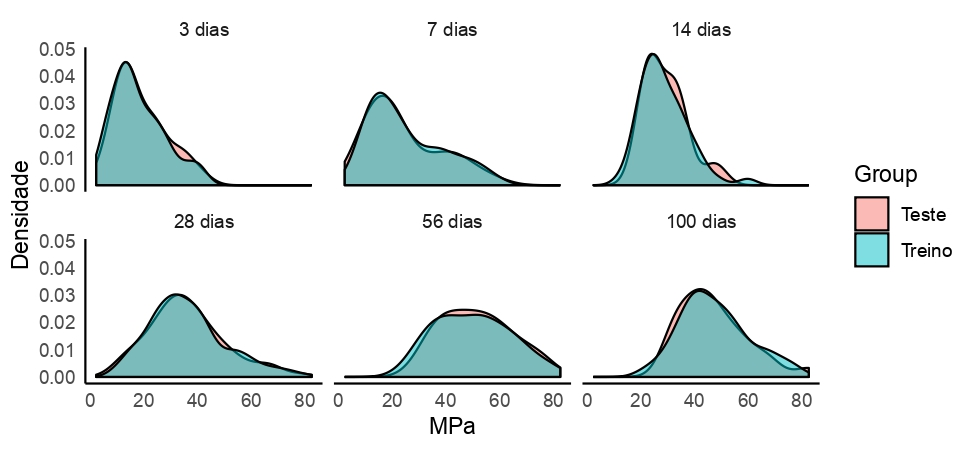
\includegraphics[scale=0.9]{Figures/dist-split_PT.jpg}
\vspace{12pt}
\caption{Distribuição dos conjuntos de teste e treino em relação à resistência à compressão}
\label{fig:split-dist}
\end{center}
\end{figure}
\vspace{8pt}


% --------------------------------------------------------------------------
\subsection{Modelos ingênuos} \label{subsec:naivemodels}
% --------------------------------------------------------------------------

Antes de construir os modelos reais, para fins de comparação, foram criados modelos ingênuos. Eles simplesmente prevêem que a resistência à compressão do conjunto de teste é a resistência à compressão média do conjunto de treino. Em outras palavras, os modelos ingênuos são simplesmente a melhor estimativa possível para avaliar o quão próximo / distante o modelo real está de um palpite aleatório.


% --------------------------------------------------------------------------
\subsection{Modelos de aprendizado de máquina} \label{subsec:machinelearningmodels}
% --------------------------------------------------------------------------

Utilizamos apenas um algoritmo neste trabalho, escolhido pela maior probabilidade para atingir o melhor resultado possível, de acordo com \citet{Fernandez2014}, que comparou 179 algoritmos em 121 bancos de dados diferentes, e concluiu que o mais provável de alcançar o melhor resultado possível é o {\it Parallel Random Forest}, chamado {\it prRF} no pacote {\it Caret} \cite{caret}.

Seis modelos diferentes foram construídos, um para cada faixa de idade, e as seguintes etapas foram feitas para cada modelo:


\begin{enumerate}

\item Definir o esquema de reamostragem, com método de validação cruzada repetida;

\item Definir a {\it tuning grid} para o parâmetro {\it mtry}, que é uma sequência de 1 ao número de colunas de cada conjunto de dados. Todos, exceto o de 7 dias, são iguais, visto que apenas o conjunto de 7 dias teve uma coluna removida no pré-processamento;

\item Definir o {\it seed} igual a 1, escolhido arbitrariamente para garantir reprodutibilidade. Esse {\it seed} pode ser manipulado para obter resultados mais satisfatórios, mas foi optado por não fazê-lo.

\item Fazer a transformação do pré-processamento dos dados com os métodos {\it center} e {\it scale};

\item Executar a função {\it train} do {\it Caret} com as configurações acima e modelo {\it parRF};

\end{enumerate}


% --------------------------------------------------------------------------
\section{Resultados}\label{sec:Results}
% --------------------------------------------------------------------------
A avaliação de desempenho dos modelos foi realizada pelo erro de raiz quadrada média ({\it RMSE}). O {\it RMSE} é a medida utilizada em todos os trabalhos citados na introdução permitindo a comparação dos modelos na discussão.

O {\it RMSE} de teste para cada modelo em ordem crescente de idade foi 3,31, 4,36, 4,62, 4,72, 5,94 e 5,85, respectivamente. A tabela  \ref{tab:results} apresenta os detalhes e resultados de cada modelo, inclusive o ingênuo. A Fig.  \ref{fig:results} compara os valores reais e previstos para os modelos finais.

\vspace{8pt}
\begin{table}[!ht]
\centering
\caption{Resultados dos modelos finais}
\label{tab:results}
\vspace{6pt}
\begin{tabular}{ccccccc}
\hline
Modelo & {\it mtry} & {\it CV} &  Repetições & {\it RMSE} ingênuo (teste) &  {\it RMSE} final (treino) & {\it RMSE} final (teste)\\ \hline
3 dias & 6 & 30 & 10 & 9.303229 & 3.905196 & 3.310370\\
7 dias & 2 & 10 & 10 & 13.443646 & 4.475981 & 4.361987\\
14 dias & 13 & 30 & 10 & 7.593319 & 5.136687 & 4.620515\\
28 dias & 11 & 30 & 10 & 14.283824 & 5.847334 & 4.716698\\
56 dias & 8 & 30 & 10 & 12.702112 & 6.702565 & 5.939163\\
100 dias & 8 & 10 & 10 & 12.614652 & 6.381940 & 5.851088\\ \hline
\end{tabular}
\end{table}
\vspace{8pt}

\begin{figure}[!ht]
\begin{center}
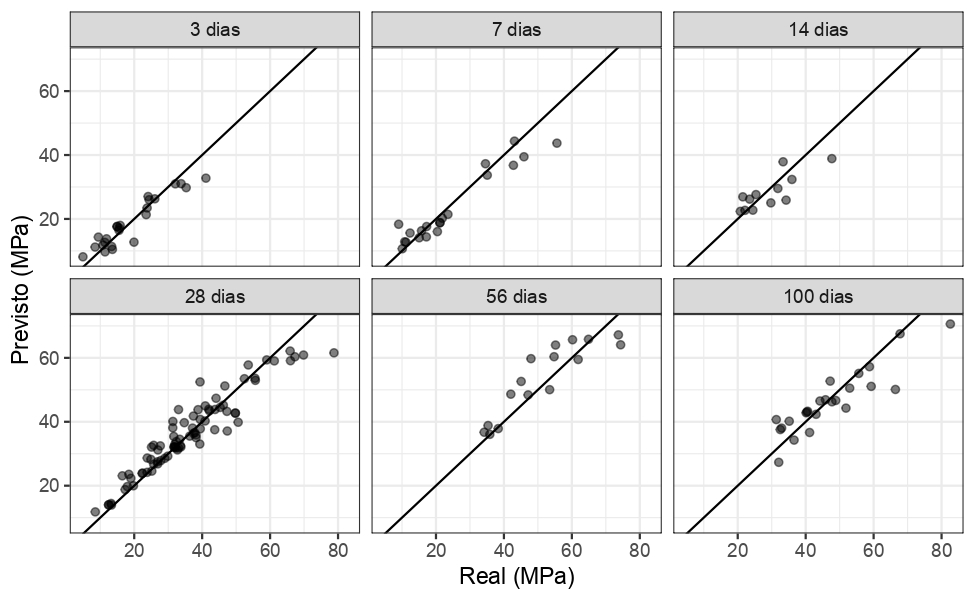
\includegraphics[scale=0.9]{Figures/results-comparison_PT.jpg}
\vspace{12pt}
\caption{Real {\it vs} previsto para cada modelo}
\label{fig:results}
\end{center}
\end{figure}
\vspace{8pt}

\pagebreak

% --------------------------------------------------------------------------
\section{Discussão e conclusão}\label{sec:DiscussionAndConclusion}
% --------------------------------------------------------------------------

Os modelos construídos apresentam resultados satisfatórios e comprovam que a resistência à compressão do concreto pode ser prevista com relativa facilidade. A alternativa adotada de criar um modelo para cada conjunto de idades mostrou-se um método válido, ao invés de usar a idade como preditor junto com os ingredientes, como realizado nos estudos relacionados com o mesmo conjunto de dados. A adoção dessa estratificação obteve resultados diferenciados para cada faixa de idade. O {\it RMSE} calculado em nosso trabalho e o obtido nos trabalhos relacionados foram próximos. A tabela \ref{tab:comparison} mostra a comparação entre esses estudos e o modelo de 28 dias aqui desenvolvido.

Seguindo a linha de raciocínio deste trabalho, a mesma hipótese pode ser avaliada utilizando outros algoritmos além do aqui utilizado  ({\it Parallel Random Forest}), pois podem apresentar resultados melhores. Outra opção é criar um {\it ensemble} de vários algoritmos, como realizado por \citet{Pierobon2018}, mas com a separação dos conjuntos de idades aqui proposta. Além disso, este estudo pode ser reproduzido com um conjunto de dados maior, idealmente com um número semelhante de amostras em cada faixa de idade e uma distribuição mais homogênea de resistência à compressão e classe de concreto, visto que na Fig. \ref{fig:categorical} mostra que esse conjunto de dados é muito inclinado para a classe de concreto entre C25 e C35.

\vspace{8pt}
\begin{table}[!ht]
\centering
\caption{Comparação com outros trabalhos com o mesmo conjunto de dados}
\label{tab:comparison}
\vspace{6pt}
\begin{tabular}{lclcc}
\hline
Autor & Ano & Algoritmo & {\it RMSE} & Diferença ({\%}) \\ \hline
\citet{Pierobon2018} & 2018 & {\it Ensemble} de 5 algoritmos & 4.150 & -12\\
\textbf{Esse trabalho (28 dias)} & \textbf{2020} & \textbf{{\it Parallel Random Forest}} & \textbf{4.717}  & \textbf{0}\\
\citet{Hameed2020} & 2020 & Redes neurais artificiais & 4.736 & 0\\
\citet{Raj2018} & 2018 & {\it Gradient Boosting Regressor} & 4.957  & +5\\
\citet{Modukuru2020} & 2020 & {\it Random Forest Regressor} & 5.080  & +8\\
\citet{Alshamiri2020} & 2020 & {\it Regularized Extreme Learning Machine} & 5.508 & +17\\
\citet{Abban2016} & 2016 & {\it SVM} com {\it Radial Basis Function Kernel} & 6.105 & +29\\ \hline
\end{tabular}
\end{table}
\vspace{8pt}


\pagebreak

%--------------------------------------------------------------------------
\vspace{20pt}
\noindent \textbf{Declaração de autoria.} Os autores confirmam que são os únicos responsáveis pela autoria deste trabalho, e que todo o material aqui incluído como parte do presente trabalho é propriedade (e autoria) dos autores, ou tem a permissão dos proprietários a serem incluídos aqui.

\bibliography{bibliography}

\end{document}
% --------------------------------------------------------------------------
